\section{User interface}
\label{uilolol}


\subsection{UI Constraint}


\begin{figure}[!htbp]
  \begin{center}
    \leavevmode
    \ifpdf
      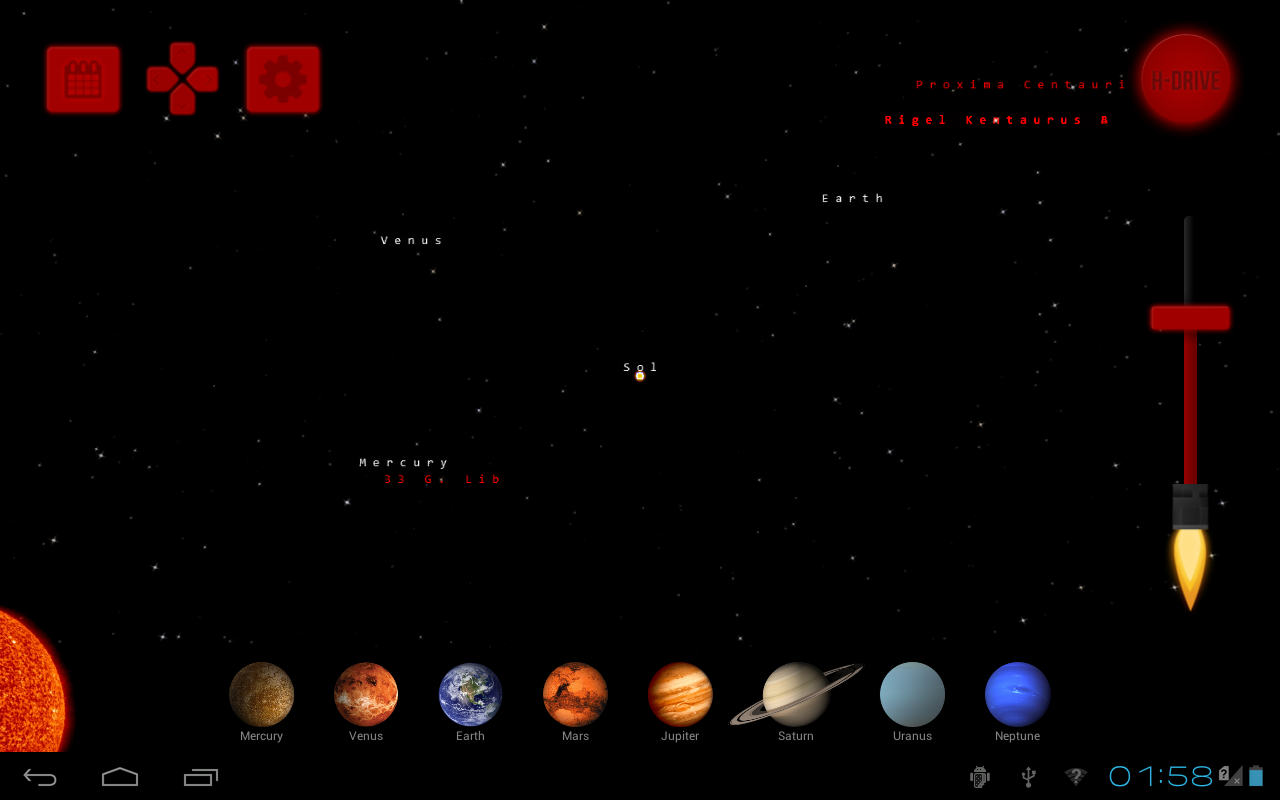
\includegraphics[width=1\textwidth]{mainuielements}
    \fi
    \caption{UI elements on main screen}
    \label{UI elements on main screen}
  \end{center}
\end{figure}

There are several factors that need to be taken into consideration in designing the controls given that the Android app mostly uses touch controls. The elements need to be big enough for its functionality to be clearly apparent, responsive on touch and to prevent the user from tapping the wrong button or missing the button, which would make it seem unresponsive. However, given that screen space on mobile devices are limited, they need to be small enough such the controls do not take attention away from the content of the app. 
\\\\\
We achieved this by first putting all the controls on the sides, which makes is much easier for the user to focus on the content in the centre, and by providing small buttons to show and hide the bigger elements. If by default we showed all the controls on the screen: the full calendar, the keypad and all the planets, there would be almost no space left for the content.


\subsection{Main UI elements walkthrough}


\subsubsection{Accelerator}

\begin{figure}[!htbp]
  \begin{center}
    \leavevmode
    \ifpdf
      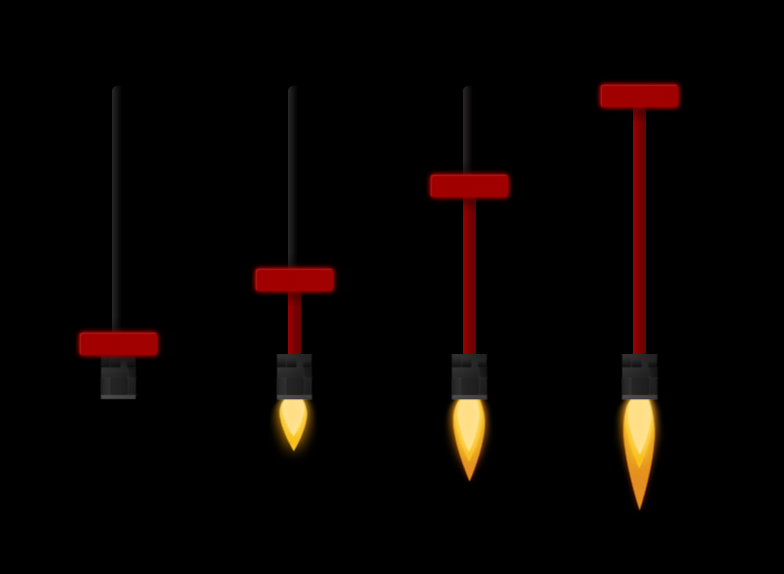
\includegraphics[width=1\textwidth]{accelerator_dif_states}
    \fi
    \caption{Accelerator at different levels}
    \label{Accelerator at different levels}
  \end{center}
\end{figure}

The speed of the camera can be controlled by the user with sliders. To add extra visual feedback, the size of the flames varies with speed.



\subsubsection{Hyperjump to planets}

\begin{figure}[h!]
  \begin{center}
    \leavevmode
    \ifpdf
      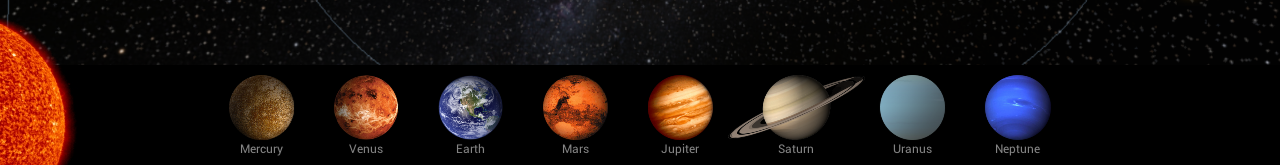
\includegraphics[width=1\textwidth]{hyperjump_planets}
    \fi
    \caption{Hyperjump planets selector}
    \label{Hyperjump planets selector}
  \end{center}
\end{figure}

\begin{figure}[!htbp]
  \begin{center}
    \leavevmode
    \ifpdf
      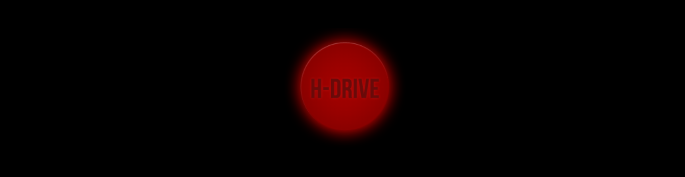
\includegraphics[width=1\textwidth]{hyperjump_button.png}
    \fi
    \caption{Hyperjump button}
    \label{Hyperjump button}
  \end{center}
\end{figure}

The icons of planets at the bottom of the app for hyperjump appears when the Hyperjump button is pressed or when the app is started. When a planet is touched, the camera focusses on this particular planet.

\subsection{Secondary UI elements walkthrough}
\subsubsection{Gamepad}

\begin{figure}[!htbp]
  \begin{center}
    \leavevmode
    \ifpdf
      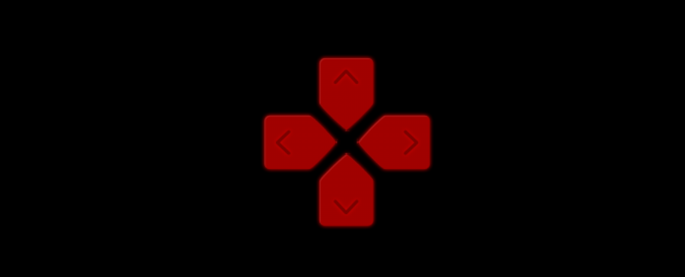
\includegraphics[width=1\textwidth]{gamepad}
    \fi
    \caption{Gamepad}
    \label{Gamepad}
  \end{center}
\end{figure}

By default the direction of the ship is given by finger gestures; swiping in the opposite direction of desired movement. However, the user may also want to pan across the screen to have a different perspective of a planet, so we need extra controls to do that. The full size gamepad appears when the user taps on the gamepad icon, to save screen space as previously mentioned.

\subsubsection{Calendar}

\begin{figure}[!htbp]
  \begin{center}
    \leavevmode
    \ifpdf
      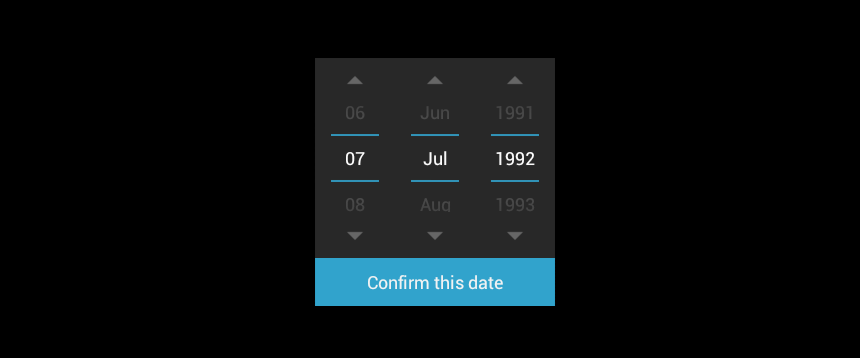
\includegraphics[width=1\textwidth]{calendar}
    \fi
    \caption{Calendar}
    \label{Calendar}
  \end{center}
\end{figure}

The calendar lets you select a date and see the simulation at this particular point in time. The calendar appears when we tap on the calendar icon.

\subsubsection{Select different simulation modes}

\begin{figure}[!htbp]
  \begin{center}
    \leavevmode
    \ifpdf
      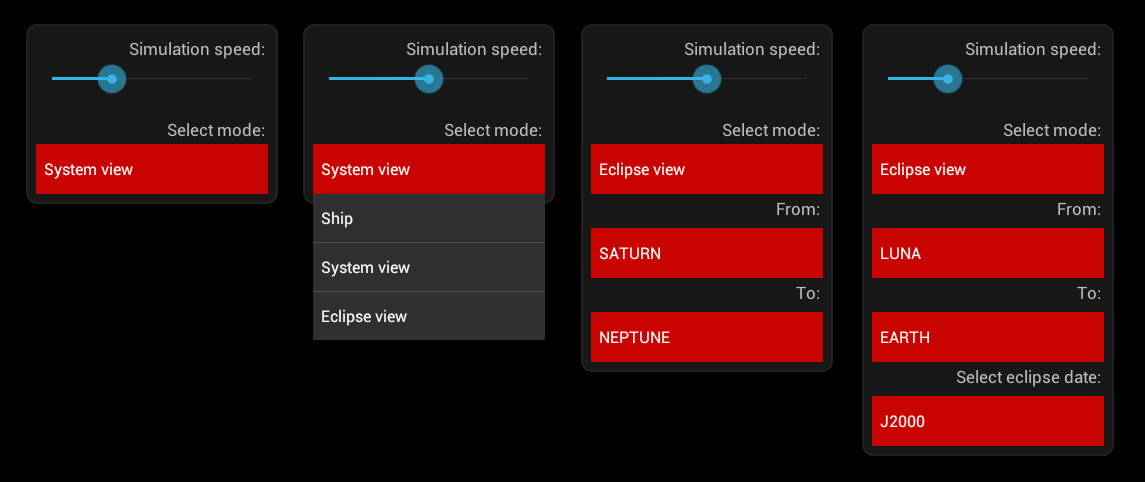
\includegraphics[width=1\textwidth]{states_modes}
    \fi
    \caption{Different states for selecting modes}
    \label{Different states for selecting modes}
  \end{center}
\end{figure}

There are three different modes for the simulation: Ship, System View and Eclipse View. To easily swich between those modes and set specific parameters for the Eclipse mode, extra elements can be made available by tapping on the Settings icon. 

\subsection{Android UI coding}

The easiest way to display elements on an android app is to add those elements to a .xml layout file. Android has a collection of default elements we can use.

\subsubsection{ImageView}

The most used element in the UI, we use the ImageView markup and specify an image path, and other options like the size, position. Almost all the ImageViews in the project also have a onClick parameter, that allows us to call a specific function when the image is touched on an android device.
\\\\
So for example, we have defined an ImageView for the calendar icon, with the image path pointing to the icon we created on Photoshop and then exported, and it calls a function that will show or hide the full calendar when touched.

\subsubsection{HorizontalScrollView}

The app must be able to run on a variety of Android devices, with a wide range of resolutions. If the width of the device is not large enough, all the planet icons at the bottom of the screen for hyperjump will not fit, and the user will not be able to access all the planets. Using a HorizontalScrollView solves this problem as this area becomes scrollable and the hidden icons can be reached. Similar to the ImageView, we can specify paramaters like height, width, position, and also background color. Inside a HorizontalScrollView we can put any UI elements we want; images, text, tables, etc.

\subsubsection{TextView}

Then we have TextViews. They are used to display the names below the planet icons for hyperjump and in the box to select different modes. We can change the font, color, size, position and other formatting.

\subsubsection{SeekBar}

\begin{figure}[!htbp]
  \begin{center}
    \leavevmode
    \ifpdf
      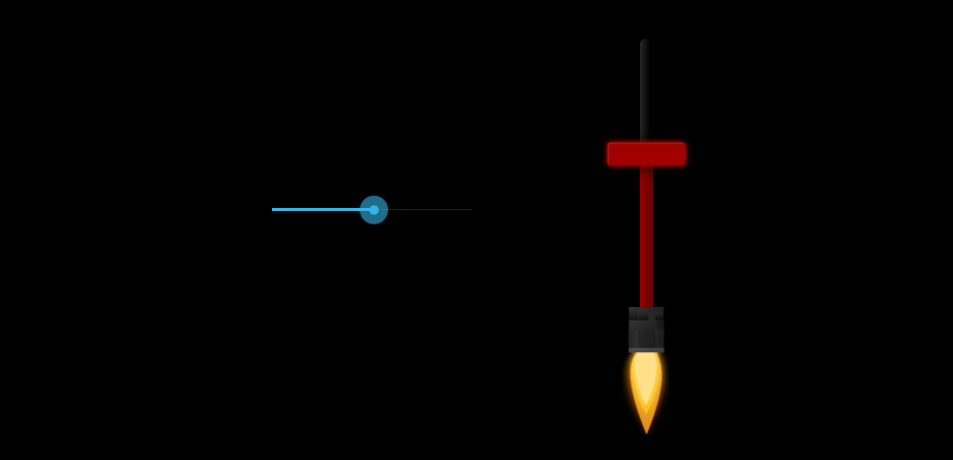
\includegraphics[width=1\textwidth]{seekbarvsreactor}
    \fi
    \caption{Regular Android SeekBar vs modified SeekBar}
    \label{Regular Android SeekBar vs modified SeekBar}
  \end{center}
\end{figure}

There are two SeekBars; one to change the speed of the simulation in the \emph{modes box}, for which we just defined the position, size and max value, and the other to alter the speed of the ship. This SeekBar had to be modified from the Android collection; first it had to be rotated 90 degrees and then we had to overwrite the progress bar in red with a gradient, the empty progress bar in black with gradient, the rounded corners of the progress bar, and the slider. When the value of the SeekBar changes, a function is called; we use this to change the size of the flame of the reactor: the reactor is actually an ImageView and according to the value of the SeekBar we change the path of the ImageView to the correct flame size. 

\subsubsection{LinearLayout and TableLayout}
LinearLayout and TableLayout are used to position elements on top of each other. TableLayout allows for more complex layouts but for basic positioning can be done by both.

\subsubsection{Spinner}

Spinners, more commonly known as drop-down lists, are used to enable the user select the different modes, planets and dates in Eclipse mode. We define them in the .xml layout file and then we populate them with all the possible choices.


















